\documentclass[conference]{IEEEtran}
\IEEEoverridecommandlockouts
\usepackage{amsmath,amssymb,amsfonts}
\usepackage{algorithmic}
\usepackage{graphicx}
\usepackage{textcomp}
\usepackage{xcolor}
\def\BibTeX{{\rm B\kern-.05em{\sc i\kern-.025em b}\kern-.08em
    T\kern-.1667em\lower.7ex\hbox{E}\kern-.125emX}}
\begin{document}

\title{Robot Navigation in a Simulated Escape Room}

\author{Gianluca Viviano \quad Etienne Orio \quad Sara Mashhadi Alizadeh}

\maketitle

\begin{abstract}
This report describes an autonomous robot system built for a
simulated escape-room task.
A DJI RoboMaster~EP robot, running in CoppeliaSim, must explore
an unknown room, find a coloured key cylinder, pick it up, and
place it on a pressure plate.
The robot uses only wheel-encoder odometry, a 2D lidar scan,
and a monocular camera.
We built three components on top of ROS~2, Nav2, and slam\_toolbox:
a lidar sensor script injected into the simulator, a colour-based
landmark detector using monocular depth estimation, and a nine-state
mission controller that combines Nav2 path planning with
visual servoing for the pickup.
The robot reliably completes all tested scenarios from start to finish.
\end{abstract}


% =====================================================================
\section{Introduction}

This project is an escape-room task in simulation.
A DJI RoboMaster~EP robot is placed in a room with obstacles and
must find a magenta cylinder (the key), pick it up, and drop it on
a green pressure plate to finish.
The room layout and object positions are not known in advance.

\begin{figure}[htbp]
\centerline{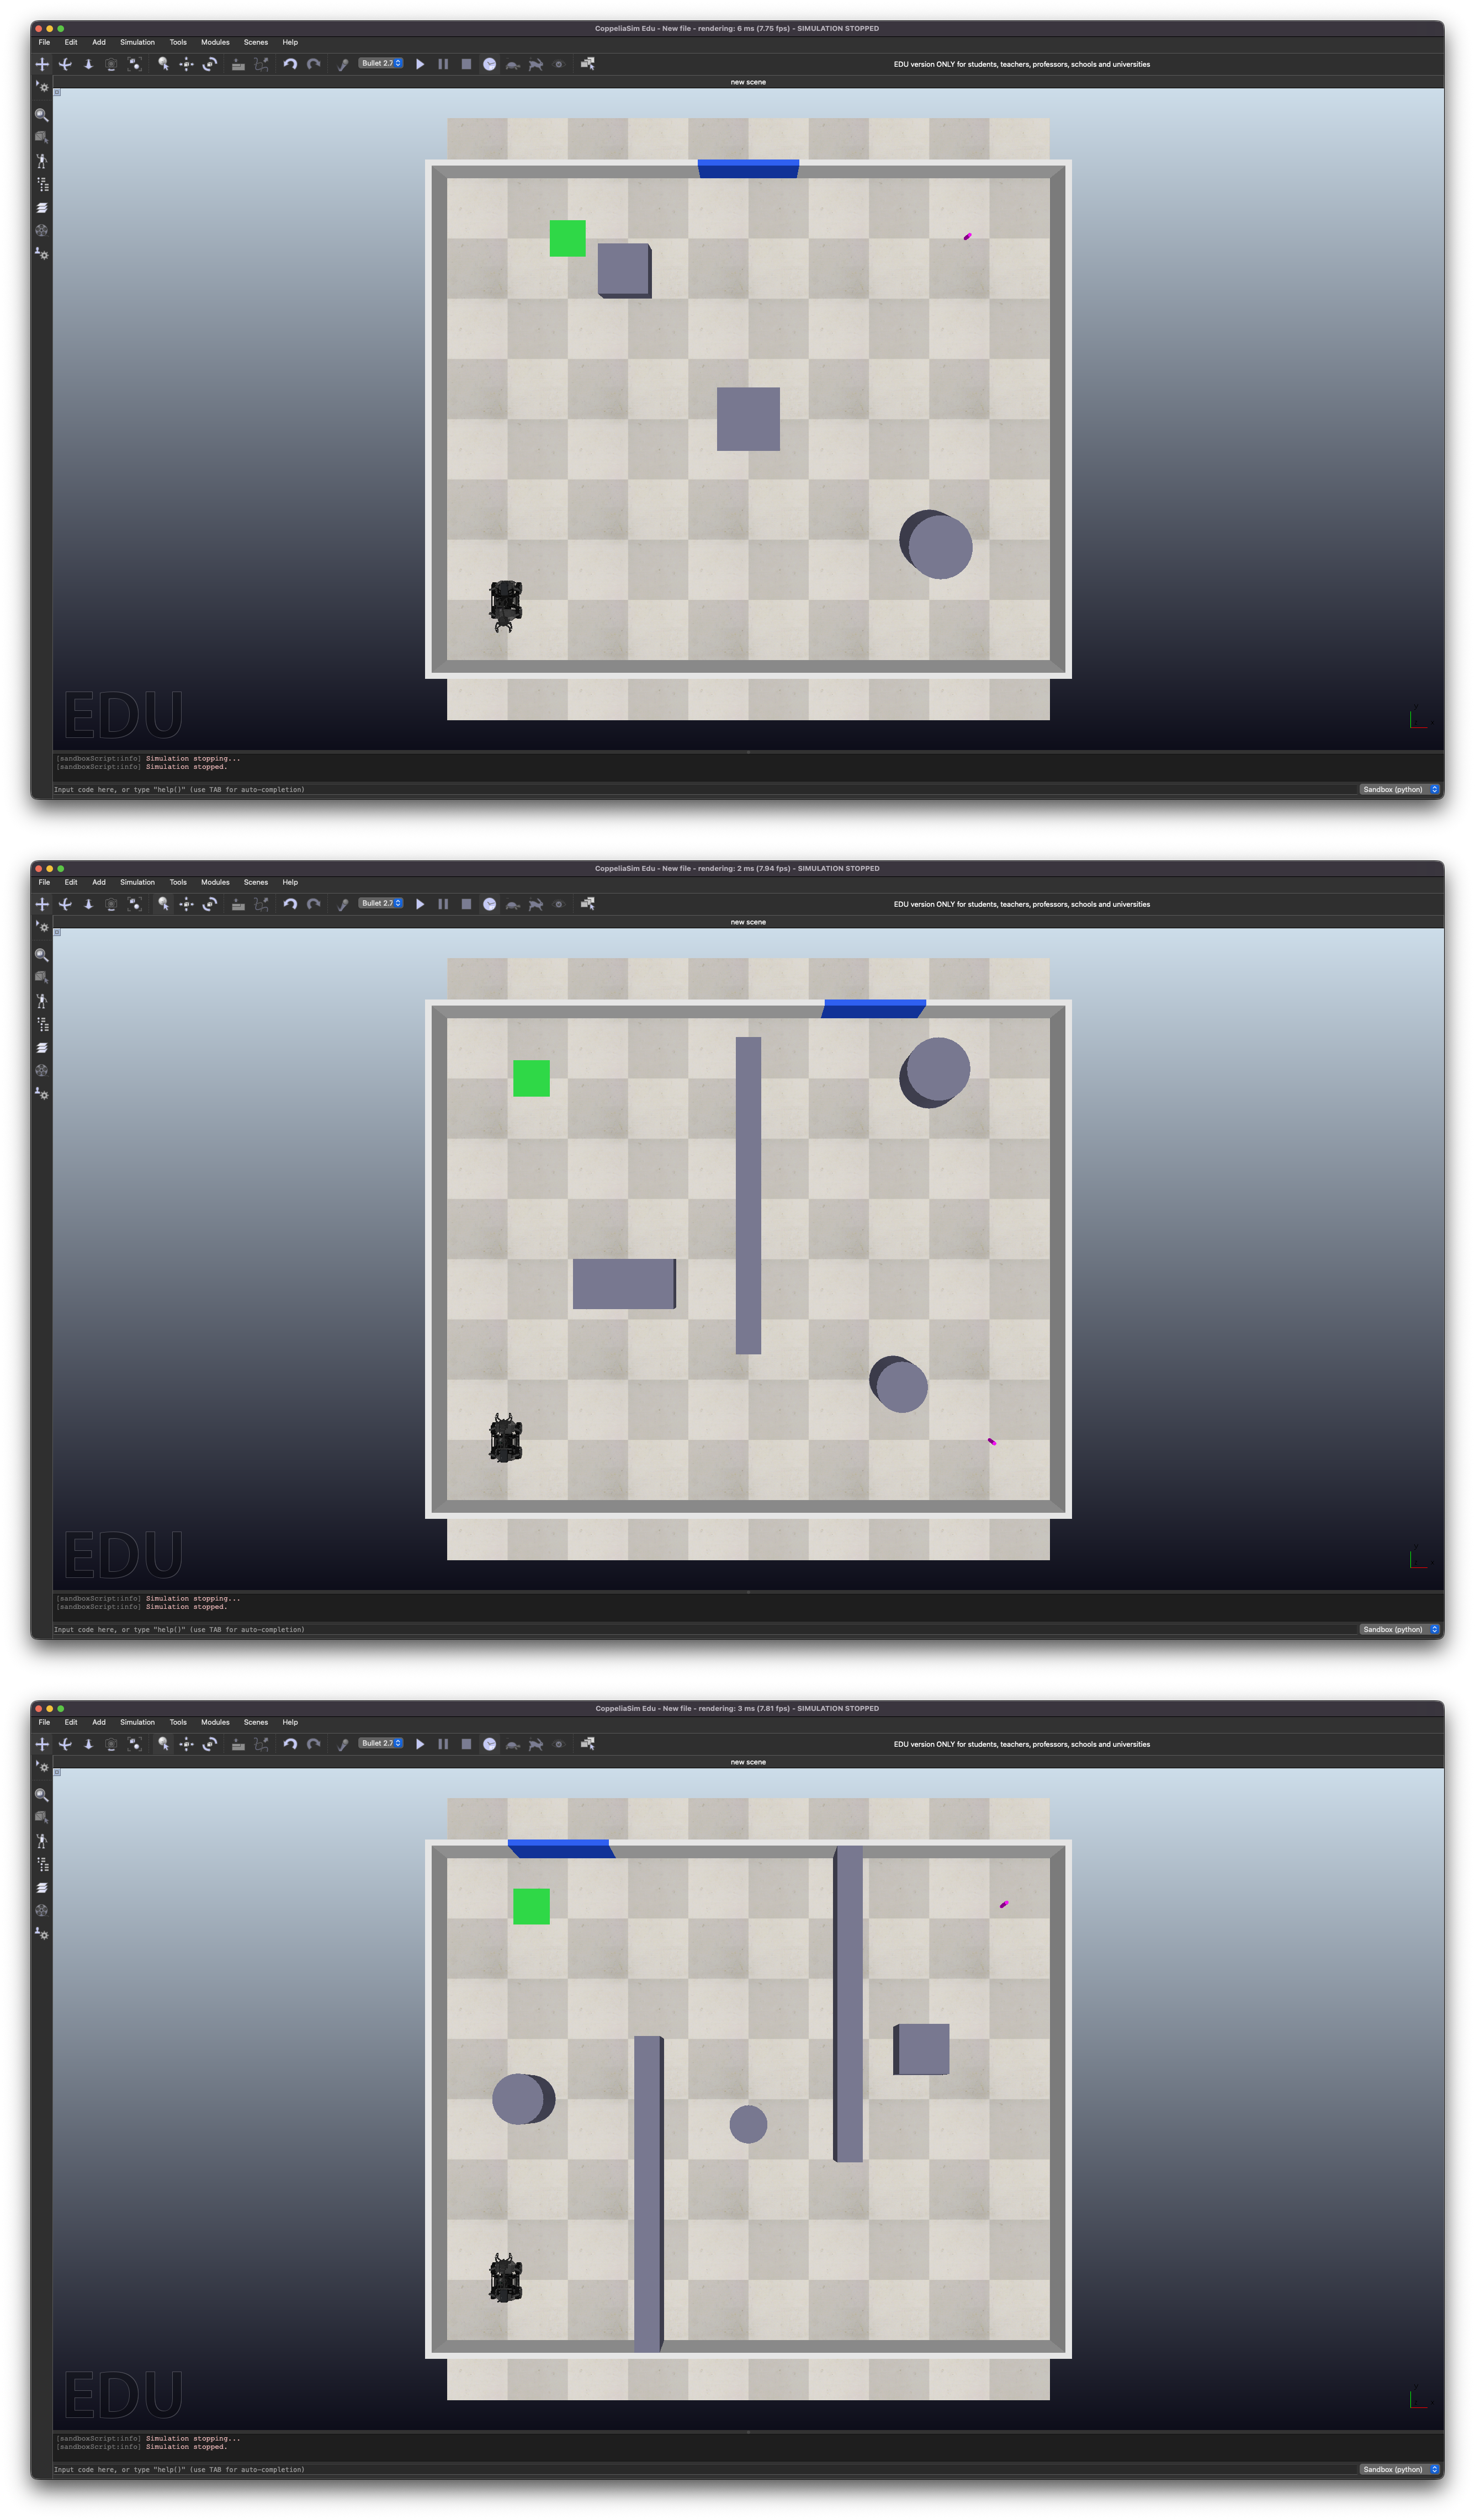
\includegraphics[width=\columnwidth]{fig_scenarios.png}}
\caption{The three scenario variants (easy, medium, hard) shown
from above in CoppeliaSim. Obstacle count and placement increase
across scenarios; the robot spawn, key, and plate positions also
change.}
\label{fig:scenarios}
\end{figure}

The simulation runs in CoppeliaSim with the
\texttt{robomaster\_sim} plugin and \texttt{robomaster\_ros} driver.
We built three custom components on top of
\texttt{slam\_toolbox} and Nav2:
a lidar sensor, a colour detector, and a mission controller.

The rest of this report is structured as follows.
Section~\ref{sec:arch} explains the overall system.
Sections~\ref{sec:perception}--\ref{sec:mission} describe each component.
Section~\ref{sec:challenges} covers the problems we ran into and how
we fixed them.
Section~\ref{sec:conclusion} concludes.

% =====================================================================
\section{System Architecture}
\label{sec:arch}

\subsection{Node graph and data flow}

Fig.~\ref{fig:arch} shows the data flow between all nodes.
The system has two custom ROS~2 nodes on top of the standard
Nav2 and \texttt{slam\_toolbox} stacks.
\texttt{color\_detector\_node} subscribes to the raw camera image,
runs the HSV pipeline, and publishes a latched
\texttt{PoseStamped} for each detected landmark on
\texttt{/targets/\{cube,plate,door\}}; it also streams the live
cube bearing on \texttt{/targets/cube\_live} at every frame for
the visual-servo phase.
\texttt{explorer\_node} is the mission FSM: it subscribes to
the target poses and the occupancy map, drives long-range
navigation by sending \texttt{NavigateToPose} goals to Nav2,
and takes direct \texttt{cmd\_vel} control for the short-range
pickup and drop manoeuvres.

\begin{figure}[htbp]
\centerline{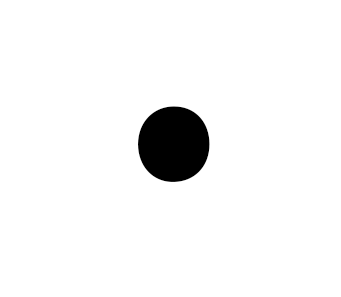
\includegraphics[width=\columnwidth]{fig_architecture.png}}
\caption{Node graph. White boxes: our components. Grey: third-party packages.
Arrows show the main ROS~2 topics and actions between nodes.}
\label{fig:arch}
\end{figure}

\subsection{Scenario configuration}

The room, obstacles, and task objects are all defined in a JSON file
that is passed to the scene builder at startup.
The file contains: room size and wall thickness; door openings;
a list of obstacles (type, position, size, colour); the key cylinder;
and the pressure plate.
The scene builder connects to CoppeliaSim, removes any previous
objects, and builds the room from scratch.
This means changing the scenario only requires swapping the JSON file,
no code changes are needed.
Three scenarios are included: \texttt{easy.json} (5$\times$4~m room,
three obstacles), \texttt{medium.json} (same room, four obstacles
with a wall-length divider, offset door, and different robot start),
and \texttt{hard.json} (increased obstacle density and a more
constrained layout).
The colours in the JSON must match the HSV thresholds in the
colour detector.

\subsection{Simulator--ROS bridge}

CoppeliaSim exposes a ZMQ-based remote API that lets external programs
call simulator functions as Python method calls at runtime, without
any shared memory or special ROS bridge.
We use it in three places.
A scene-building script (\texttt{build\_scene.py}) uses the API to
build the room from the scenario file at startup.
The colour detector reads the camera field-of-view angle once at
startup to compute the focal length for depth estimation.
The mission controller opens and closes the gripper, and toggles
the cube's \emph{detectable} flag to hide it from the lidar while it
is being carried, preventing Nav2 from mapping the held cube as a
wall directly in front of the robot.


% =====================================================================
\section{Perception}
\label{sec:perception}

\subsection{Lidar sensor}

CoppeliaSim does not publish laser scans for ROS~2 by default.
We wrote a Lua script that is injected into the simulator at startup
and attached to the robot.
Each cycle (10~Hz) the script rotates a ray sensor through 360
uniformly spaced angles, reads the hit distance, and publishes
the result as a laser scan.
The robot body is made invisible to the ray sensor so that rays
pass through the chassis and only hit walls and obstacles.

\subsection{Colour landmark detection}

To find the three landmarks (cube, plate, door), the colour detector
processes each camera frame in HSV colour space.
For each target it applies a colour mask, finds connected blobs, and
keeps the largest one that exceeds a minimum size.
The colour ranges used are: cube (magenta, $H \in [140,170]$),
plate (green, $H \in [40,80]$), door (blue, $H \in [100,130]$)
(OpenCV convention, $H \in [0,179]$).
Magenta was chosen for the cube because it does not appear in the
floor or wall textures of the simulation.

\begin{figure}[htbp]
\centerline{
\includegraphics[width=\columnwidth]{fig_camera_blob.png}}
\caption{Camera view with HSV blob detection. Coloured overlays show
the detected regions for the cube (magenta), pressure plate (green),
and door (blue). The centroid of each blob is used to estimate
the object's position.}
\label{fig:blob}
\end{figure}

\subsubsection{Depth from known height (cube and door)}

The cube and door are upright objects with known real heights
(0.20~m and 0.50~m).
The pinhole camera model gives depth directly from the blob's pixel
height: an object that is $H$ metres tall and appears $h_\mathrm{px}$
pixels tall is at depth $z = f H / h_\mathrm{px}$, where $f$ is the
focal length derived from the camera's field-of-view angle read from
the simulator at startup.
The blob centroid is then back-projected to that depth in the camera
frame and transformed into the map frame via the TF tree.
Frames where the blob touches the image edge are skipped because the
visible pixel height is cut off and would give a wrong depth.

\subsubsection{Floor-ray intersection (pressure plate)}

The plate is flat on the floor, so its pixel height gives no useful
depth.
Instead, we cast a ray through the centroid pixel, transform the ray
into the map frame, and intersect it with the floor plane ($z = 0$)
to recover the plate's $(x, y)$ position.
This approach works regardless of the plate's size and requires no
knowledge of the plate dimensions.


% =====================================================================
\section{Navigation and Mapping}
\label{sec:nav}

\subsection{SLAM}

\texttt{slam\_toolbox} runs in online mapping mode and builds a 2D
occupancy map at 5~cm per cell from the lidar scan and odometry.
Scan matching aligns each new scan against the current map, correcting
the accumulated wheel-slip drift that raw odometry alone cannot
account for on the RoboMaster's mecanum drive.
We disabled loop closure because in this small room it caused
sudden jumps of 0.3--0.5~m in the \texttt{map}$\to$\texttt{odom}
transform when the robot revisited a mapped area, which caused Nav2 to
abort its current goal mid-path.
Without loop closure the drift over one exploration pass is small
enough (sub-cell) to complete the task reliably.

\begin{figure}[htbp]
\centerline{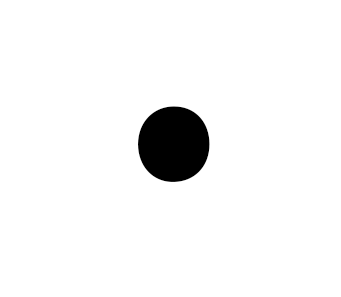
\includegraphics[width=\columnwidth]{fig_map.png}}
\caption{Occupancy grid map built by slam\_toolbox during exploration.
White cells are free space, black cells are obstacles, and grey is
unexplored. The planned path from Nav2 is shown in green.}
\label{fig:map}
\end{figure}

\subsection{Nav2}

Nav2 handles all long-range path planning and following.
We use the NavFn planner (Dijkstra) with a 0.5~m \emph{planner}
tolerance (the maximum distance between the computed path endpoint
and the requested goal), and the Regulated Pure Pursuit (RPP)
controller at a target speed of 0.15~m/s.
RPP was preferred over the DWB controller because it has fewer
parameters to tune and produces smooth, predictable trajectories at
the low speeds dictated by the small room.
A separate \emph{goal checker} with a 0.25~m position tolerance
determines when the \texttt{NavigateToPose} action reports success.
The local costmap is a 2$\times$2~m rolling window with 0.35~m
inflation around obstacles.
The global costmap covers the full map.

\subsection{Frontier exploration}

To explore the room the robot uses frontier-based exploration.
A frontier cell is a free cell (map value 0) with at least one
unknown neighbour (map value $-1$).
Adjacent frontier cells are grouped into clusters by BFS;
clusters with fewer than 20 cells are discarded as noise.
Each tick the robot sends a \texttt{NavigateToPose} goal to Nav2 for
the closest cluster centre, so the same planner and controller handle
both exploration driving and task navigation.
Exploration stops once all three landmarks have been detected; at
that point the FSM cancels any active Nav2 goal and transitions to
\textbf{GO\_TO\_KEY}.

% =====================================================================
\section{Mission Execution}
\label{sec:mission}

\subsection{State machine overview}

\begin{figure}[htbp]
\centerline{
\includegraphics[width=\columnwidth]{fig_fsm.png}}
\caption{Mission state machine. Shaded states use Nav2 for driving;
white states use direct velocity commands.}
\label{fig:fsm}
\end{figure}

The mission controller (Fig.~\ref{fig:fsm}) runs as a timer callback
at 4~Hz. It waits at startup until Nav2, the occupancy map, and the
robot's position in the map frame are all available, then advances
through ten states:
\begin{enumerate}
  \item \textbf{EXPLORE}
  \item \textbf{GO\_TO\_KEY}
  \item \textbf{PICKUP\_OPEN}
  \item \textbf{PICKUP\_ALIGN}
  \item \textbf{PICKUP\_CLOSE}
  \item \textbf{GO\_TO\_PLATE}
  \item \textbf{DROP\_ALIGN}
  \item \textbf{DROP\_OPEN}
  \item \textbf{DROP\_BACKUP}
  \item \textbf{DONE}
\end{enumerate}

\subsection{Exploration and navigation to key}

\textbf{EXPLORE}: the robot sends \texttt{NavigateToPose} goals to
the nearest frontier cluster centroid (Section~\ref{sec:nav}).
Each time a landmark is detected by the colour detector its pose is
stored; the state ends as soon as all three landmarks (cube, plate,
door) have been seen at least once and their poses are known.

\begin{figure}[htbp]
\centerline{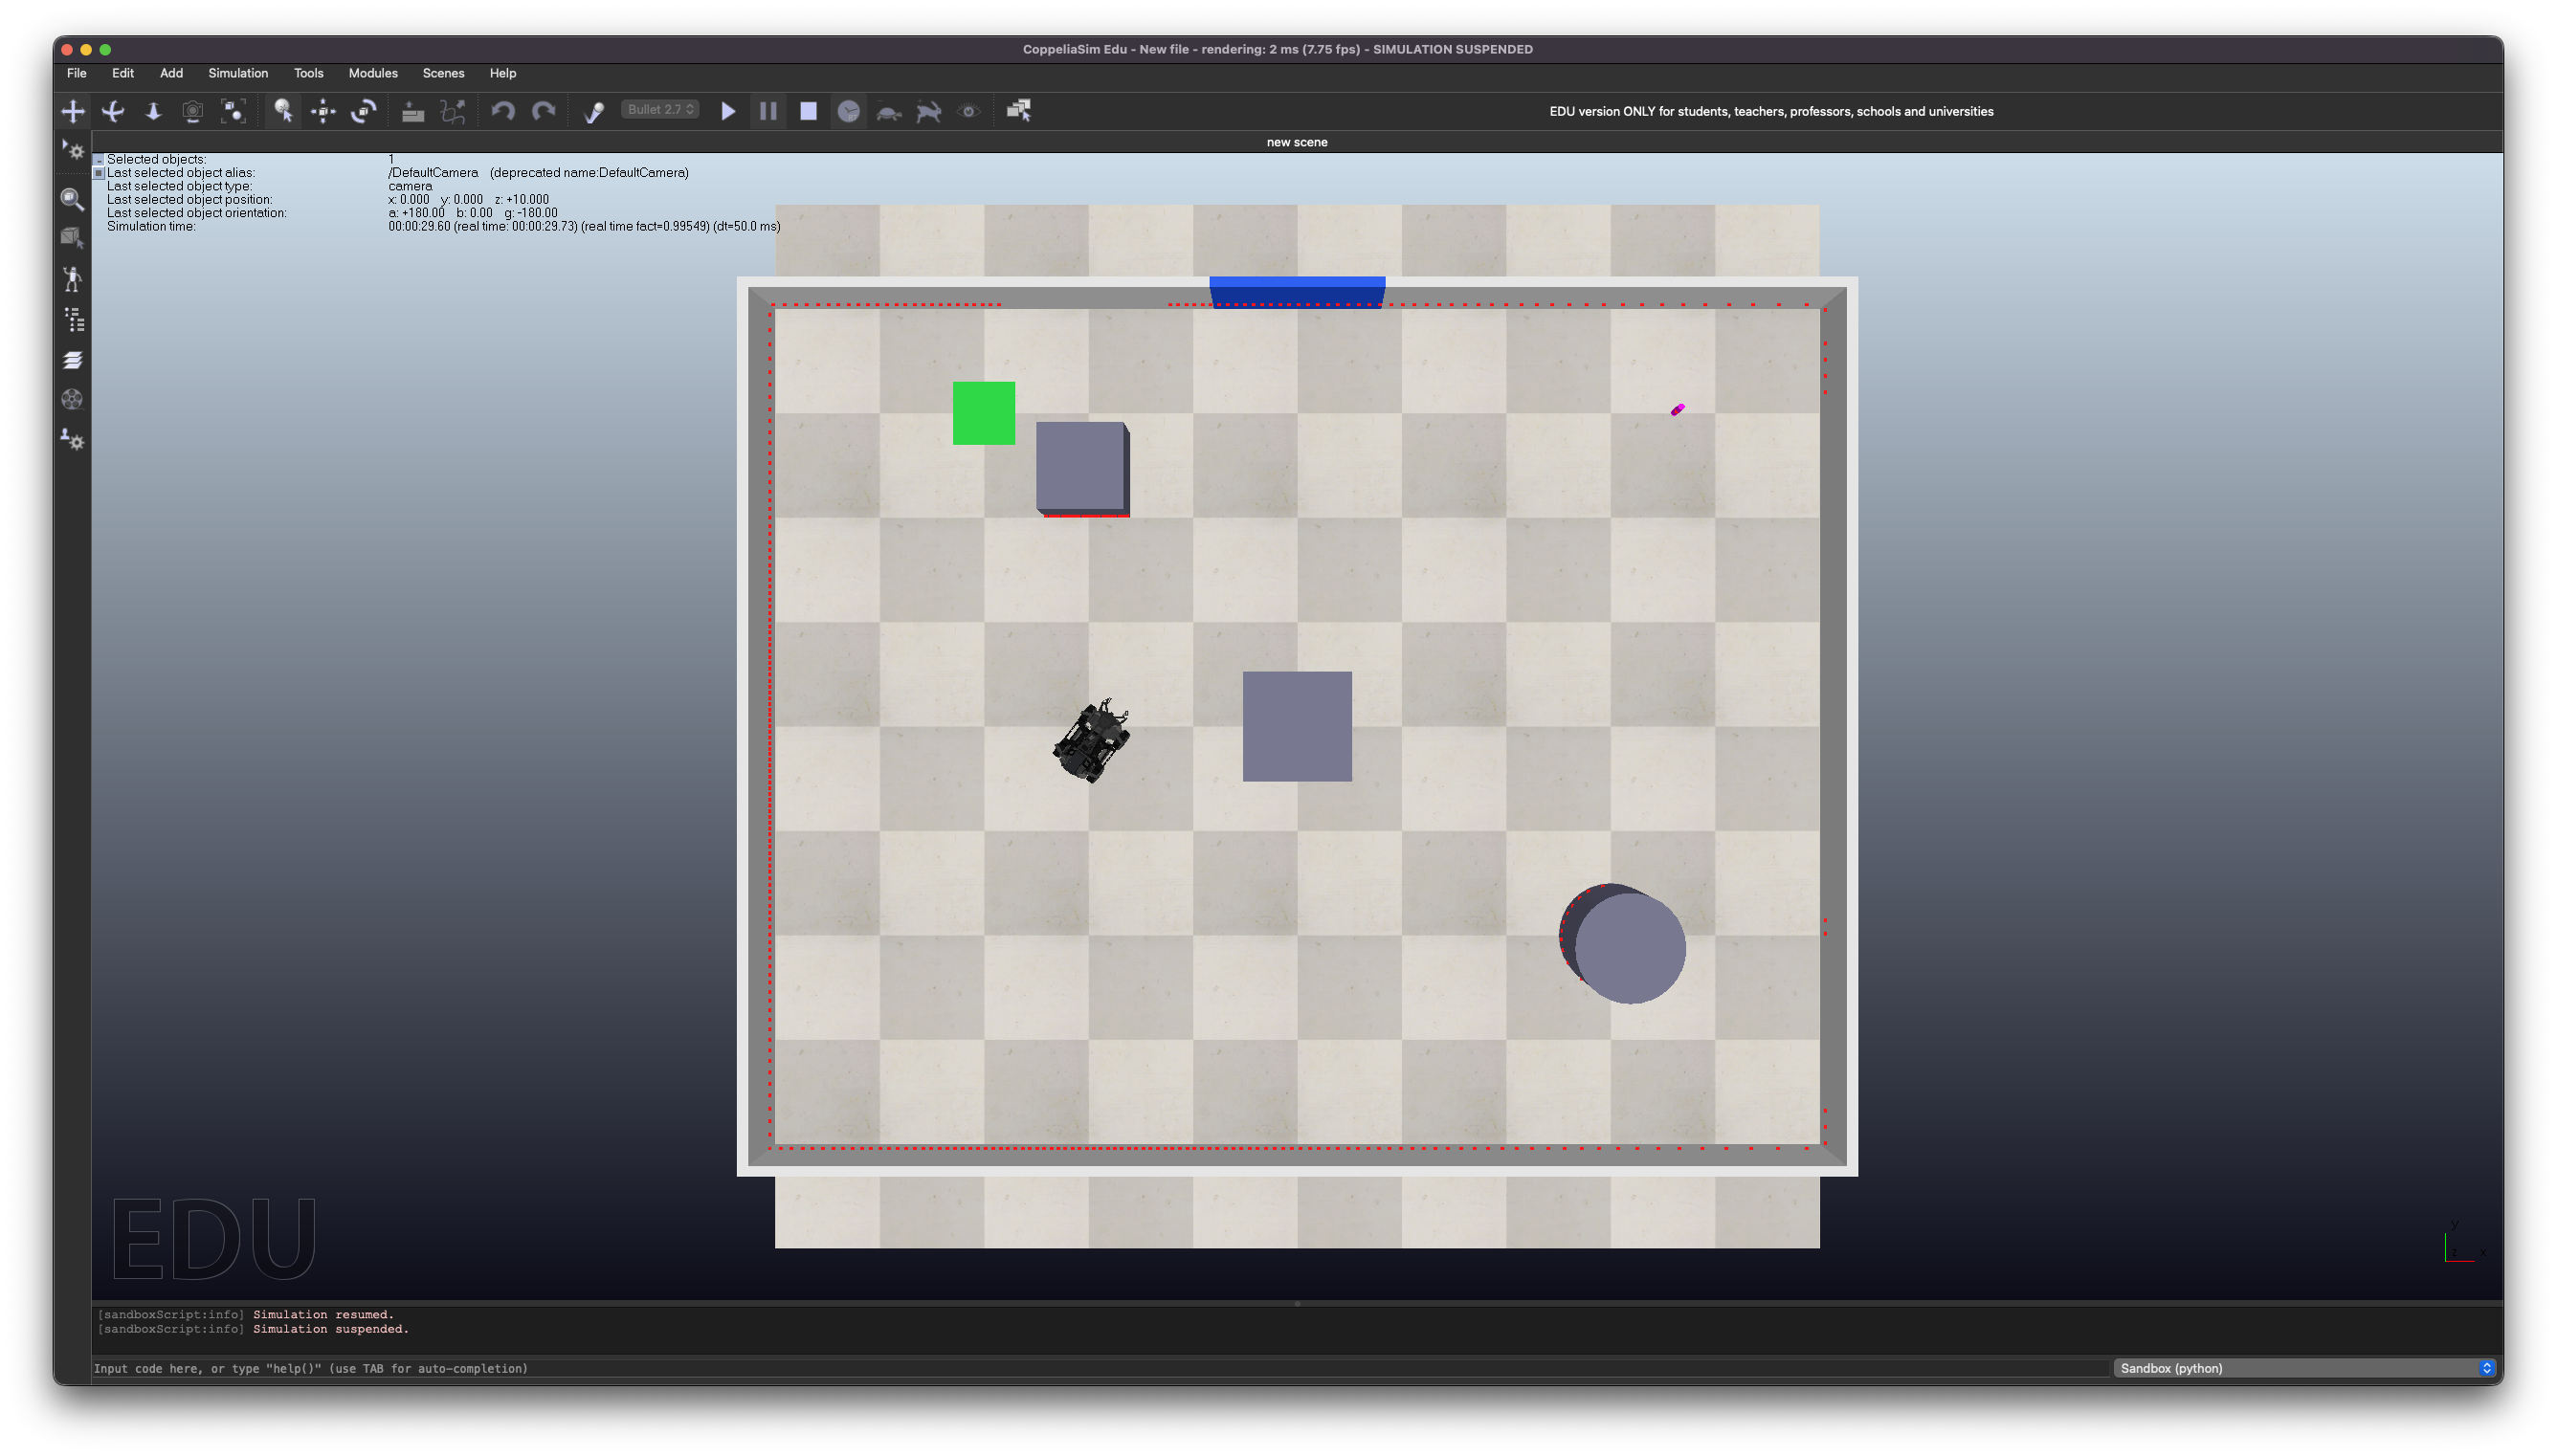
\includegraphics[width=\columnwidth]{fig_stage_explore.png}}
\caption{EXPLORE state: the robot drives toward the nearest frontier
while slam\_toolbox builds the map. The planned path and current
costmap are visible in RViz.}
\label{fig:stage_explore}
\end{figure}

\textbf{GO\_TO\_KEY}: Nav2 drives the robot to a standoff point 0.9~m
in front of the cube, oriented to face it.
Stopping 0.9~m away gives the visual-servo phase enough working range
before the cylinder base leaves the camera's field of view.
If Nav2 reports failure the goal is retried automatically.

\subsection{Pickup sequence}

\textbf{PICKUP\_OPEN}: commands the gripper to open fully and waits
for confirmation before advancing.

\textbf{PICKUP\_ALIGN}: the most complex state.
The robot uses the live cube bearing from \texttt{/targets/cube\_live}:
a proportional controller on yaw error turns the robot to keep the
cube centred in the image while driving forward.
At about 0.9~m the base of the 0.20~m cylinder moves below the
camera's lower edge, making the pixel-height depth estimate
unreliable.
The robot freezes the last valid range reading and switches to an
\emph{odometry lunge}: it drives straight ahead by
$d_\mathrm{lunge} = r - d_\mathrm{engage} - d_\mathrm{margin}$,
where $r = 0.9$~m, $d_\mathrm{engage} = 0.177$~m is the gripper
reach, and $d_\mathrm{margin} = 0.03$~m avoids tipping the cylinder.
Odometry is used instead of the SLAM transform because short
straight-line odometry is smooth and accurate, whereas the
\texttt{map}$\to$\texttt{odom} transform can jump.

\textbf{PICKUP\_CLOSE}: closes the gripper and waits for confirmation.
The cube is then hidden from the lidar
(\texttt{objectspecialproperty\_detectable\_all = 0}) so that Nav2
does not see the carried object as a wall in front of the robot.

\begin{figure}[htbp]
\centerline{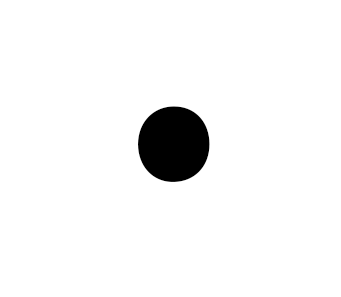
\includegraphics[width=\columnwidth]{fig_stage_pickup.png}}
\caption{PICKUP\_ALIGN state: the robot approaches the magenta
cylinder using visual servoing. The camera view (inset) shows the
cube centred in the frame just before the odometry lunge.}
\label{fig:stage_pickup}
\end{figure}

\subsection{Drop sequence}

\textbf{GO\_TO\_PLATE}: Nav2 drives the robot to the plate position
stored during exploration.
The same retry logic as GO\_TO\_KEY applies.
Because the plate is flat on the floor and does not obstruct the
lidar, Nav2 can plan and drive directly to it.

\begin{figure}[htbp]
\centerline{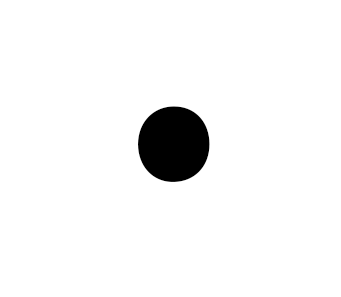
\includegraphics[width=\columnwidth]{fig_stage_drop.png}}
\caption{DROP\_OPEN state: the cube has been placed on the green
pressure plate. The robot is backing away before turning.}
\label{fig:stage_drop}
\end{figure}

\textbf{DROP\_ALIGN}: the controller switches to direct \texttt{cmd\_vel}.
Proportional control on yaw error faces the robot toward the plate,
then drives it forward until the cube's estimated position
($d_\mathrm{carried} = 0.207$~m ahead of \texttt{base\_link})
is within 0.03~m of the plate centre.

\textbf{DROP\_OPEN}: the gripper opens and the cube's lidar visibility
is restored so the map reflects its new position on the plate.

\textbf{DROP\_BACKUP}: the robot reverses 0.25~m in a straight line
measured by odometry before allowing any turning.
Turning with an open gripper would sweep the cube off the plate.

\textbf{DONE}: the mission controller stops issuing commands and the
robot remains stationary.

% =====================================================================
\section{Engineering Challenges}
\label{sec:challenges}

\subsection{Replacing a custom stack with Nav2 and slam\_toolbox}

The first version used a script that read all object positions from
the simulator directly, published them as perfect odometry, and used
a custom Python mapper with an A* planner.
This worked but was unreliable: timing problems in the API calls
corrupted the pose, and the mapper had no scan matching.
We replaced everything with \texttt{slam\_toolbox} and Nav2, using
real wheel-encoder odometry.
This was a lot of work to configure (costmaps, controller tuning,
recovery behaviours) but gave us a much more reliable system.

\subsection{Lidar: Python node to Lua script}

The first lidar was a Python ROS~2 node that queried the simulator
for the distance to each object individually.
Because it had no access to actual object geometry, it approximated
every shape as an axis-aligned bounding box (AABB): cylinders
appeared as squares on the occupancy map, which confused Nav2's
costmap and planner.
We replaced it with a Lua script running inside the simulator that
rotates a native ray sensor and reads hit distances directly from
the physics engine.
The ray sensor sees actual geometry, so cylinders map as circles
and any scene works without knowing the object list in advance.

\subsection{Loop closure jumping}

With loop closure enabled, \texttt{slam\_toolbox} sometimes applied a
large correction to the map transform when the robot revisited a
known area.
This moved the robot's estimated position by 0.3--0.5~m instantly,
which made Nav2 abort its current goal.
We disabled loop closure.
The map quality did not noticeably worsen in this small room.

\subsection{Pickup: waypoint to visual servo to odometry lunge}

The first pickup strategy drove to a fixed position offset from the
cube's known location.
The gripper missed often because the position estimate was off by
5--10~cm.
We switched to visual servoing, which keeps the cube centred in the
camera during the approach and does not depend on map accuracy.

We then found a second problem: below 0.9~m, the cylinder base
disappears from the camera's view, making the depth estimate
unreliable.
We added the odometry lunge to handle this last stretch, where
odometry is accurate enough for the short straight-line distance
involved.

\subsection{Gripper: friction-only hold}

The stock gripper script calls \texttt{sim.setObjectParent} to attach
the grasped object rigidly to the gripper's scene-graph node, which
means the cube's orientation is locked to the gripper and any rotation
during driving would tilt it off the plate on release.
The scene builder comments out that call directly in the gripper
script source before the simulation starts, so the cube is held
purely by contact forces instead.
To make friction-only holding reliable we raised the friction
coefficient to 1.0 on the gripper fingers and the cube across all
supported physics engines, and added linear and angular damping to
the cube to prevent bouncing or spinning when the gripper closes.

\subsection{Removing the GO\_TO\_DOOR state}

We originally included a \textbf{GO\_TO\_DOOR} state that drove the
robot through the door after placing the cube on the plate.
In testing, the monocular depth estimate for the door
(height 0.50~m) had positional errors of 15--20~cm at the approach
distances required for navigation.
The door opening is only 0.80~m wide, so that error margin made
reliable passage through the doorway impossible without repeated
replanning.
We removed the state entirely: the door is detected during
exploration to count as one of the three required landmarks, but the
mission ends at \textbf{DONE} once the cube is on the plate.

\subsection{CoppeliaSim real-time mode watchdog}

The \texttt{robomaster\_sim} plugin uses a 3-second
\emph{simulation-time} heartbeat watchdog.
Without real-time mode, CoppeliaSim advances roughly $3\times$ faster
than wall clock, so the driver's 1~Hz heartbeat times out in about
one real second, silently dropping \texttt{/odom}, \texttt{/imu},
and all chassis topics for the rest of the run, while the simulator
itself continued normally.
The failure mode was a robot that stopped moving partway through
exploration with no error in the ROS log.
The fix was to call
\texttt{sim.setBoolParam(\allowbreak boolparam\_realtime\_simulation,~True)}
before starting the simulation, which is handled in \texttt{run.sh}.

% =====================================================================
\section{Conclusion}
\label{sec:conclusion}

We built an autonomous robot system that solves a simulated
escape-room task: it explores an unknown room, finds three
colour-coded objects, picks up the key cylinder with visual
servoing, and drops it on the pressure plate.

The system successfully completed all three scenario variants in
testing.
Exploration and navigation were reliable across runs; the most
sensitive step was the visual-servo pickup, which occasionally
struggled when the cube was placed close to a wall and the approach
angle was narrow.
The drop alignment was more consistent because it uses direct
position control rather than camera-based depth estimation.

The main lesson is that using an existing stack (Nav2 and
slam\_toolbox) is much better than building a custom planner,
even though configuring it took significant effort.
The visual-servo pickup and the odometry lunge were necessary to
make the manipulation reliable, because map-based position estimates
were not accurate enough close to the object.

Future improvements could include better recovery when the cube is
dropped during transport, support for multi-room layouts, or a
depth camera to make the pickup more robust.

\end{document}
